\documentclass[12pt,a4paper]{article}
\usepackage[utf8]{inputenc}
\usepackage[T1]{fontenc}
\usepackage{geometry}
\usepackage{graphicx}
\usepackage{booktabs}
\usepackage{longtable}
\usepackage{hyperref}
\usepackage{enumitem}
\usepackage{xcolor}
\usepackage{fancyhdr}
\usepackage{tikz}
\usepackage{pgfgantt}
\usetikzlibrary{shapes.geometric, arrows.meta, positioning, fit, backgrounds, calc}

\geometry{margin=1in}
\pagestyle{fancy}
\fancyhf{}
\rhead{Medcare-Pharmacy Management Application}
\lhead{Documentation}
\rfoot{Page \thepage}

\title{\textbf{Medcare-
		Pharmacy Management Application}\\
\large Technical Documentation}
\author{Project Documentation}
\date{\today}

\begin{document}

\maketitle
\tableofcontents
\newpage

%=============================================================================
\section{Project Overview}
%=============================================================================

The \textbf{Medcare-Pharmacy Management Application} is a full-stack web application designed to facilitate online pharmacy operations. It provides a platform for customers to browse, search, and purchase pharmaceutical products online with secure payment processing.

\subsection{Key Features}
\begin{itemize}
    \item User registration and authentication with JWT tokens
    \item Product catalog with categories (medicines, healthcare products)
    \item Shopping cart functionality with quantity management
    \item Secure payment integration via Stripe
    \item Order management and tracking
    \item Contact form for customer inquiries
    \item Prescription upload functionality
    \item Admin capabilities for product and order management
    \item Responsive design for mobile and desktop
\end{itemize}

\subsection{Architecture}
The application follows a \textbf{MERN Stack} architecture:
\begin{itemize}
    \item \textbf{MongoDB} -- NoSQL database for data storage
    \item \textbf{Express.js} -- Backend web framework
    \item \textbf{React.js} -- Frontend library for UI
    \item \textbf{Node.js} -- Server-side JavaScript runtime
\end{itemize}

\newpage
%=============================================================================
\section{System Diagrams}
%=============================================================================

\subsection{Use Case Diagram}

The Use Case diagram illustrates the interactions between actors (Customer and Admin) and the system functionalities.

\begin{figure}[h!]
\centering
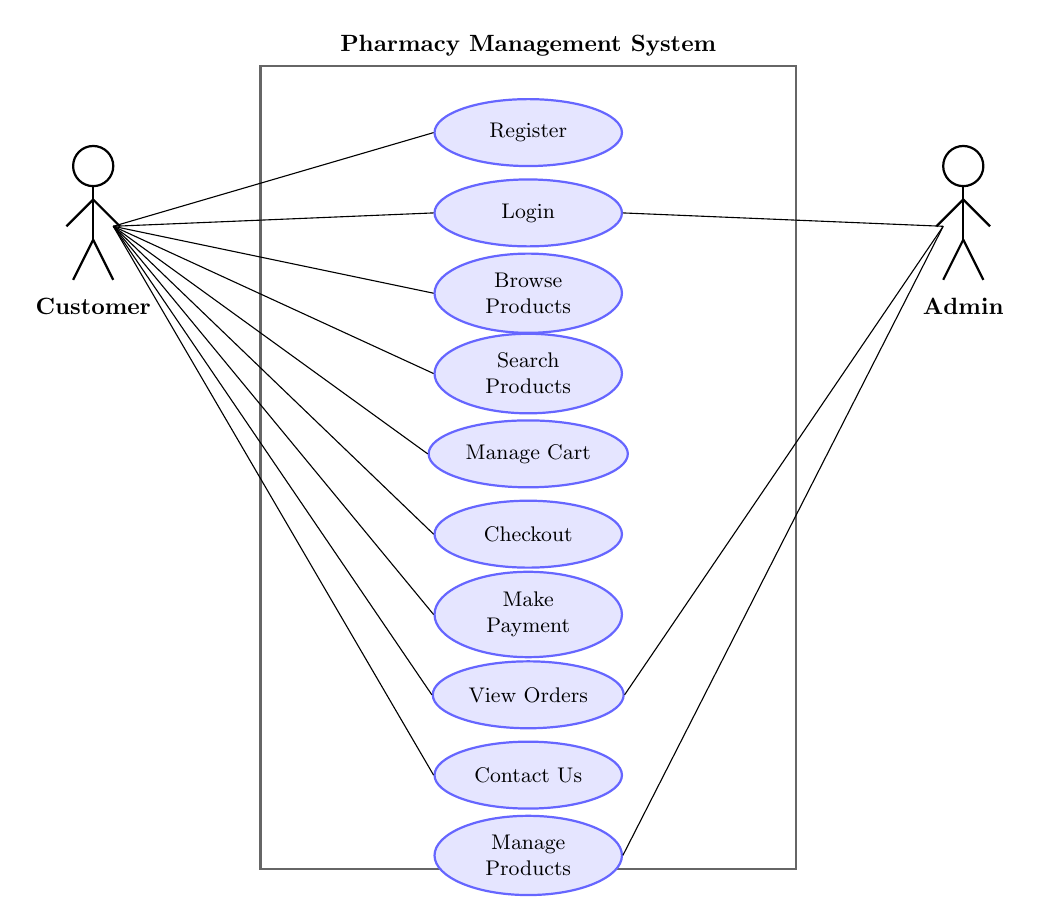
\begin{tikzpicture}[scale=0.85, transform shape]
    % Define styles
    \tikzstyle{actor} = []
    \tikzstyle{usecase} = [ellipse, draw=blue!60, fill=blue!10, thick, minimum width=2.8cm, minimum height=1cm, align=center, font=\small]
    \tikzstyle{system} = [rectangle, draw=black!60, thick, minimum width=8cm, minimum height=12cm]
    
    % System boundary
    \node[system, label={[font=\bfseries]above:Pharmacy Management System}] (system) at (5,0) {};
    
    % Customer stick figure
    \draw[thick] (-1.5, 4.5) circle (0.3cm); % head
    \draw[thick] (-1.5, 4.2) -- (-1.5, 3.4); % body
    \draw[thick] (-1.5, 4) -- (-1.9, 3.6); % left arm
    \draw[thick] (-1.5, 4) -- (-1.1, 3.6); % right arm
    \draw[thick] (-1.5, 3.4) -- (-1.8, 2.8); % left leg
    \draw[thick] (-1.5, 3.4) -- (-1.2, 2.8); % right leg
    \node[font=\bfseries] at (-1.5, 2.4) {Customer};
    
    % Admin stick figure
    \draw[thick] (11.5, 4.5) circle (0.3cm); % head
    \draw[thick] (11.5, 4.2) -- (11.5, 3.4); % body
    \draw[thick] (11.5, 4) -- (11.1, 3.6); % left arm
    \draw[thick] (11.5, 4) -- (11.9, 3.6); % right arm
    \draw[thick] (11.5, 3.4) -- (11.2, 2.8); % left leg
    \draw[thick] (11.5, 3.4) -- (11.8, 2.8); % right leg
    \node[font=\bfseries] at (11.5, 2.4) {Admin};
    
    % Use Cases - Customer side
    \node[usecase] (register) at (5, 5) {Register};
    \node[usecase] (login) at (5, 3.8) {Login};
    \node[usecase] (browse) at (5, 2.6) {Browse\\Products};
    \node[usecase] (search) at (5, 1.4) {Search\\Products};
    \node[usecase] (cart) at (5, 0.2) {Manage Cart};
    \node[usecase] (checkout) at (5, -1) {Checkout};
    \node[usecase] (payment) at (5, -2.2) {Make\\Payment};
    \node[usecase] (orders) at (5, -3.4) {View Orders};
    \node[usecase] (contact) at (5, -4.6) {Contact Us};
    
    % Admin-only use cases
    \node[usecase] (manage) at (5, -5.8) {Manage\\Products};
    
    % Customer connections
    \draw[-] (-1.2, 3.6) -- (register.west);
    \draw[-] (-1.2, 3.6) -- (login.west);
    \draw[-] (-1.2, 3.6) -- (browse.west);
    \draw[-] (-1.2, 3.6) -- (search.west);
    \draw[-] (-1.2, 3.6) -- (cart.west);
    \draw[-] (-1.2, 3.6) -- (checkout.west);
    \draw[-] (-1.2, 3.6) -- (payment.west);
    \draw[-] (-1.2, 3.6) -- (orders.west);
    \draw[-] (-1.2, 3.6) -- (contact.west);
    
    % Admin connections
    \draw[-] (11.2, 3.6) -- (login.east);
    \draw[-] (11.2, 3.6) -- (manage.east);
    \draw[-] (11.2, 3.6) -- (orders.east);
    
\end{tikzpicture}
\caption{Use Case Diagram}
\end{figure}

\newpage
\subsection{Data Flow Diagram (DFD) - Level 0}

The Context Diagram (Level 0 DFD) shows the system as a single process with external entities.

\begin{figure}[h!]
\centering
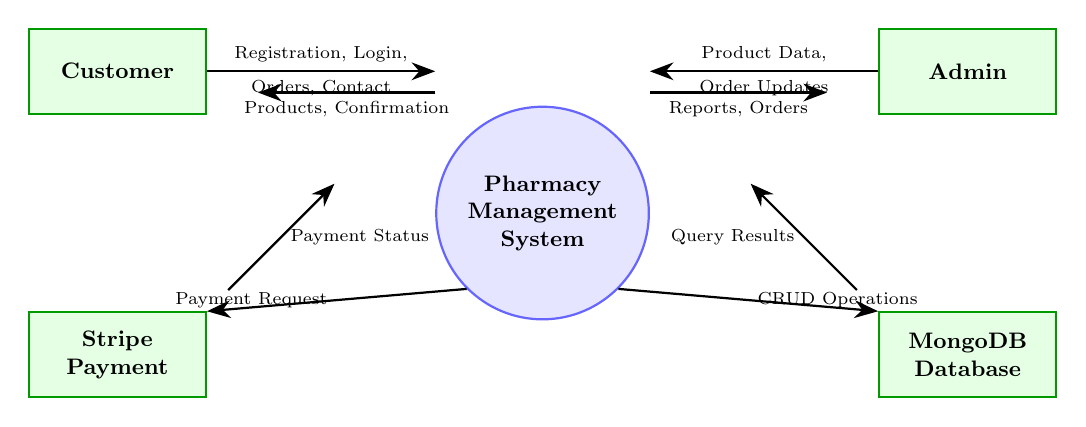
\begin{tikzpicture}[scale=0.9, transform shape]
    % Define styles
    \tikzstyle{entity} = [rectangle, draw=green!60!black, fill=green!10, thick, minimum width=2.5cm, minimum height=1.2cm, align=center, font=\small\bfseries]
    \tikzstyle{process} = [circle, draw=blue!60, fill=blue!10, thick, minimum size=3cm, align=center, font=\small\bfseries]
    \tikzstyle{arrow} = [-{Stealth[length=3mm]}, thick]
    
    % Central Process
    \node[process] (system) at (0,0) {Pharmacy\\Management\\System};
    
    % External Entities
    \node[entity] (customer) at (-6, 2) {Customer};
    \node[entity] (admin) at (6, 2) {Admin};
    \node[entity] (stripe) at (-6, -2) {Stripe\\Payment};
    \node[entity] (database) at (6, -2) {MongoDB\\Database};
    
    % Data flows - Customer
    \draw[arrow] (customer.east) -- node[above, font=\scriptsize] {Registration, Login,} node[below, font=\scriptsize] {Orders, Contact} (system.west |- customer.east);
    \draw[arrow] (system.west |- customer.east) ++(0,-0.3) -- ++(-2.5,0) node[below, font=\scriptsize, pos=0.5] {Products, Confirmation};
    
    % Data flows - Admin
    \draw[arrow] (admin.west) -- node[above, font=\scriptsize] {Product Data,} node[below, font=\scriptsize] {Order Updates} (system.east |- admin.west);
    \draw[arrow] (system.east |- admin.west) ++(0,-0.3) -- ++(2.5,0) node[below, font=\scriptsize, pos=0.5] {Reports, Orders};
    
    % Data flows - Stripe
    \draw[arrow] (system.south west) -- node[left, font=\scriptsize] {Payment Request} (stripe.north east);
    \draw[arrow] (stripe.north east) ++(0.3,0.3) -- ++(1.5,1.5) node[right, font=\scriptsize, pos=0.5] {Payment Status};
    
    % Data flows - Database
    \draw[arrow] (system.south east) -- node[right, font=\scriptsize] {CRUD Operations} (database.north west);
    \draw[arrow] (database.north west) ++(-0.3,0.3) -- ++(-1.5,1.5) node[left, font=\scriptsize, pos=0.5] {Query Results};
    
\end{tikzpicture}
\caption{Context Diagram (Level 0 DFD)}
\end{figure}

\subsection{Data Flow Diagram (DFD) - Level 1}

\begin{figure}[h!]
\centering
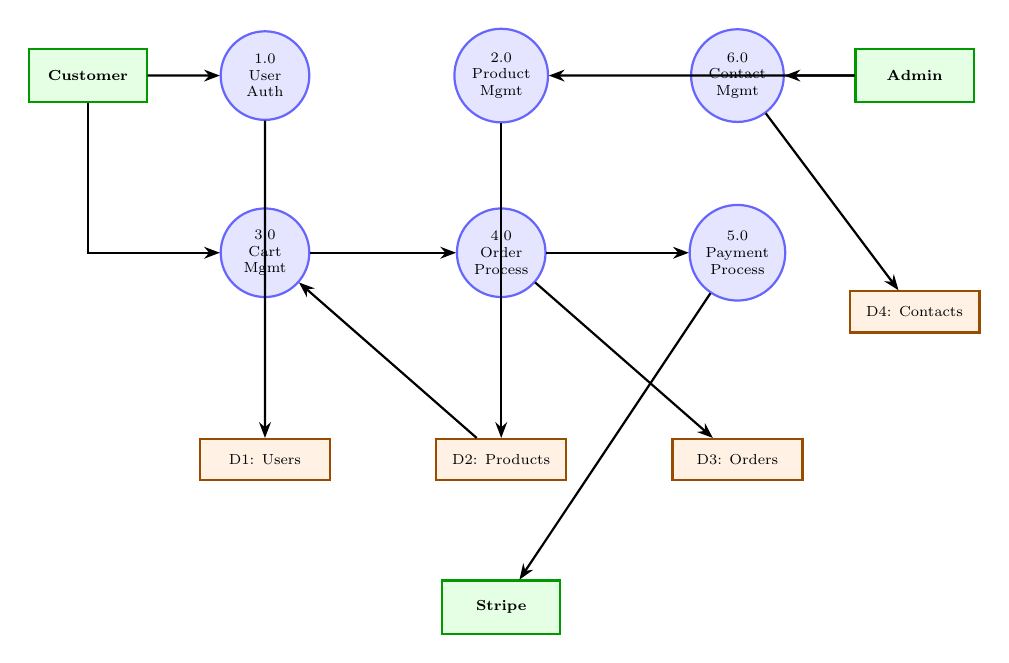
\begin{tikzpicture}[scale=0.75, transform shape]
    % Define styles
    \tikzstyle{entity} = [rectangle, draw=green!60!black, fill=green!10, thick, minimum width=2cm, minimum height=0.9cm, align=center, font=\scriptsize\bfseries]
    \tikzstyle{process} = [circle, draw=blue!60, fill=blue!10, thick, minimum size=1.5cm, align=center, font=\scriptsize]
    \tikzstyle{datastore} = [rectangle, draw=orange!60!black, fill=orange!10, thick, minimum width=2.2cm, minimum height=0.7cm, align=center, font=\scriptsize]
    \tikzstyle{arrow} = [-{Stealth[length=2mm]}, thick]
    
    % External Entities
    \node[entity] (customer) at (-7, 3) {Customer};
    \node[entity] (admin) at (7, 3) {Admin};
    \node[entity] (stripe) at (0, -6) {Stripe};
    
    % Processes
    \node[process] (p1) at (-4, 3) {1.0\\User\\Auth};
    \node[process] (p2) at (0, 3) {2.0\\Product\\Mgmt};
    \node[process] (p3) at (-4, 0) {3.0\\Cart\\Mgmt};
    \node[process] (p4) at (0, 0) {4.0\\Order\\Process};
    \node[process] (p5) at (4, 0) {5.0\\Payment\\Process};
    \node[process] (p6) at (4, 3) {6.0\\Contact\\Mgmt};
    
    % Data Stores
    \node[datastore] (d1) at (-4, -3.5) {D1: Users};
    \node[datastore] (d2) at (0, -3.5) {D2: Products};
    \node[datastore] (d3) at (4, -3.5) {D3: Orders};
    \node[datastore] (d4) at (7, -1) {D4: Contacts};
    
    % Arrows
    \draw[arrow] (customer) -- (p1);
    \draw[arrow] (p1) -- (d1);
    \draw[arrow] (customer) |- (p3);
    \draw[arrow] (p2) -- (d2);
    \draw[arrow] (p3) -- (p4);
    \draw[arrow] (p4) -- (d3);
    \draw[arrow] (p4) -- (p5);
    \draw[arrow] (p5) -- (stripe);
    \draw[arrow] (admin) -- (p2);
    \draw[arrow] (admin) -- (p6);
    \draw[arrow] (p6) -- (d4);
    \draw[arrow] (d2) -- (p3);
    
\end{tikzpicture}
\caption{Level 1 Data Flow Diagram}
\end{figure}

\newpage
\subsection{Entity-Relationship (ER) Diagram}

The ER diagram shows the database structure and relationships between entities.

\begin{figure}[h!]
\centering
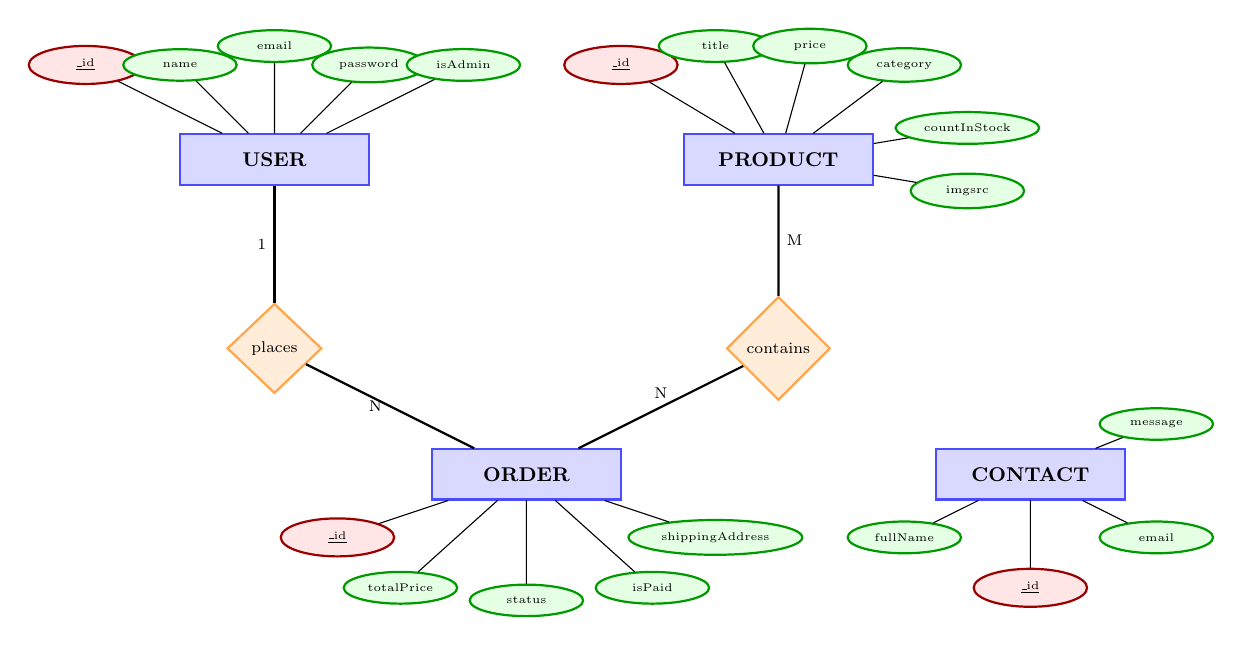
\begin{tikzpicture}[scale=0.8, transform shape]
    % Define styles
    \tikzstyle{entity} = [rectangle, draw=blue!70, fill=blue!15, thick, minimum width=3cm, minimum height=0.8cm, font=\small\bfseries]
    \tikzstyle{attribute} = [ellipse, draw=green!60!black, fill=green!10, thick, minimum width=1.8cm, minimum height=0.5cm, font=\tiny, align=center]
    \tikzstyle{key} = [ellipse, draw=red!60!black, fill=red!10, thick, minimum width=1.8cm, minimum height=0.5cm, font=\tiny, align=center]
    \tikzstyle{relation} = [diamond, draw=orange!70, fill=orange!15, thick, minimum width=1.5cm, minimum height=1cm, font=\scriptsize, align=center]
    
    % USER Entity
    \node[entity] (user) at (0, 6) {USER};
    \node[key] (uid) at (-3, 7.5) {\underline{\_id}};
    \node[attribute] (uname) at (-1.5, 7.5) {name};
    \node[attribute] (uemail) at (0, 7.8) {email};
    \node[attribute] (upass) at (1.5, 7.5) {password};
    \node[attribute] (uadmin) at (3, 7.5) {isAdmin};
    
    \draw (user) -- (uid);
    \draw (user) -- (uname);
    \draw (user) -- (uemail);
    \draw (user) -- (upass);
    \draw (user) -- (uadmin);
    
    % PRODUCT Entity
    \node[entity] (product) at (8, 6) {PRODUCT};
    \node[key] (pid) at (5.5, 7.5) {\underline{\_id}};
    \node[attribute] (ptitle) at (7, 7.8) {title};
    \node[attribute] (pprice) at (8.5, 7.8) {price};
    \node[attribute] (pcat) at (10, 7.5) {category};
    \node[attribute] (pstock) at (11, 6.5) {countInStock};
    \node[attribute] (pimg) at (11, 5.5) {imgsrc};
    
    \draw (product) -- (pid);
    \draw (product) -- (ptitle);
    \draw (product) -- (pprice);
    \draw (product) -- (pcat);
    \draw (product) -- (pstock);
    \draw (product) -- (pimg);
    
    % ORDER Entity
    \node[entity] (order) at (4, 1) {ORDER};
    \node[key] (oid) at (1, 0) {\underline{\_id}};
    \node[attribute] (ototal) at (2, -0.8) {totalPrice};
    \node[attribute] (ostatus) at (4, -1) {status};
    \node[attribute] (opaid) at (6, -0.8) {isPaid};
    \node[attribute] (oship) at (7, 0) {shippingAddress};
    
    \draw (order) -- (oid);
    \draw (order) -- (ototal);
    \draw (order) -- (ostatus);
    \draw (order) -- (opaid);
    \draw (order) -- (oship);
    
    % CONTACT Entity
    \node[entity] (contact) at (12, 1) {CONTACT};
    \node[key] (cid) at (12, -0.8) {\underline{\_id}};
    \node[attribute] (cname) at (10, 0) {fullName};
    \node[attribute] (cemail) at (14, 0) {email};
    \node[attribute] (cmsg) at (14, 1.8) {message};
    
    \draw (contact) -- (cid);
    \draw (contact) -- (cname);
    \draw (contact) -- (cemail);
    \draw (contact) -- (cmsg);
    
    % Relationships
    \node[relation] (places) at (0, 3) {places};
    \node[relation] (contains) at (8, 3) {contains};
    
    % Relationship lines
    \draw[thick] (user) -- node[left, font=\scriptsize] {1} (places);
    \draw[thick] (places) -- node[left, font=\scriptsize] {N} (order);
    \draw[thick] (order) -- node[above, font=\scriptsize] {N} (contains);
    \draw[thick] (contains) -- node[right, font=\scriptsize] {M} (product);
    
\end{tikzpicture}
\caption{Entity-Relationship Diagram}
\end{figure}

\newpage
\subsection{Project Timeline - Gantt Chart}

\begin{figure}[h!]
\centering
\begin{ganttchart}[
    hgrid,
    vgrid,
    x unit=0.5cm,
    y unit chart=0.6cm,
    y unit title=0.8cm,
    title height=1,
    bar height=0.6,
    bar/.append style={fill=blue!40},
    bar incomplete/.append style={fill=blue!20},
    milestone/.append style={fill=red!60},
    group/.append style={fill=green!30},
    title label font=\scriptsize\bfseries,
    bar label font=\scriptsize,
    group label font=\scriptsize\bfseries,
    milestone label font=\scriptsize
]{1}{24}
    \gantttitle{Project Development Timeline (Weeks)}{24} \\
    \gantttitlelist{1,...,24}{1} \\
    
    % Phase 1: Planning
    \ganttgroup{Phase 1: Planning}{1}{4} \\
    \ganttbar{Requirements Analysis}{1}{2} \\
    \ganttbar{System Design}{2}{3} \\
    \ganttbar{Database Design}{3}{4} \\
    \ganttmilestone{Design Complete}{4} \\
    
    % Phase 2: Backend Development
    \ganttgroup{Phase 2: Backend}{5}{12} \\
    \ganttbar{Setup Node.js/Express}{5}{6} \\
    \ganttbar{MongoDB Integration}{6}{7} \\
    \ganttbar{User Authentication}{7}{9} \\
    \ganttbar{Product API}{9}{10} \\
    \ganttbar{Order API}{10}{11} \\
    \ganttbar{Payment Integration}{11}{12} \\
    \ganttmilestone{Backend Complete}{12} \\
    
    % Phase 3: Frontend Development
    \ganttgroup{Phase 3: Frontend}{10}{18} \\
    \ganttbar{React Setup \& Redux}{10}{11} \\
    \ganttbar{UI Components}{11}{13} \\
    \ganttbar{Product Pages}{13}{15} \\
    \ganttbar{Cart \& Checkout}{15}{17} \\
    \ganttbar{User Dashboard}{17}{18} \\
    \ganttmilestone{Frontend Complete}{18} \\
    
    % Phase 4: Testing & Deployment
    \ganttgroup{Phase 4: Testing}{19}{24} \\
    \ganttbar{Unit Testing}{19}{20} \\
    \ganttbar{Integration Testing}{20}{21} \\
    \ganttbar{Bug Fixes}{21}{23} \\
    \ganttbar{Deployment}{23}{24} \\
    \ganttmilestone{Project Launch}{24}
    
\end{ganttchart}
\caption{Project Development Gantt Chart}
\end{figure}

\newpage
\subsection{System Architecture Block Diagram}

\begin{figure}[h!]
\centering
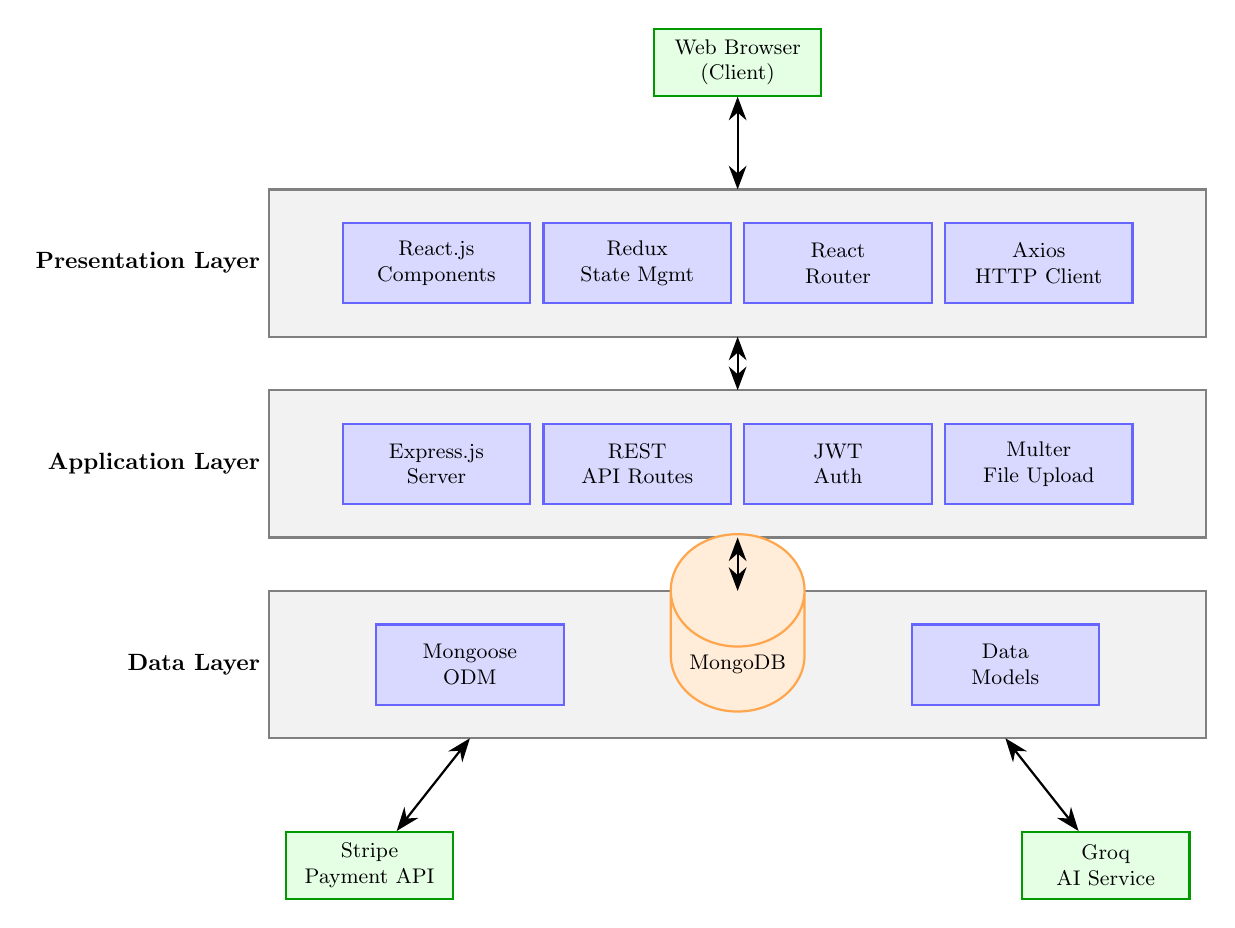
\begin{tikzpicture}[scale=0.85, transform shape]
    % Define styles
    \tikzstyle{block} = [rectangle, draw=black!70, fill=white, thick, minimum width=2.5cm, minimum height=1cm, align=center, font=\small]
    \tikzstyle{layer} = [rectangle, draw=black!50, fill=gray!10, thick, minimum width=14cm, minimum height=2.2cm, align=center]
    \tikzstyle{component} = [rectangle, draw=blue!60, fill=blue!15, thick, minimum width=2.8cm, minimum height=1.2cm, align=center, font=\small]
    \tikzstyle{database} = [cylinder, draw=orange!70, fill=orange!15, thick, shape border rotate=90, minimum width=2cm, minimum height=1.5cm, font=\small]
    \tikzstyle{external} = [rectangle, draw=green!60!black, fill=green!10, thick, minimum width=2.5cm, minimum height=1cm, align=center, font=\small]
    \tikzstyle{arrow} = [{Stealth[length=3mm]}-{Stealth[length=3mm]}, thick]
    
    % Presentation Layer
    \node[layer, label={[font=\bfseries]left:Presentation Layer}] (pres) at (0, 6) {};
    \node[component] at (-4.5, 6) {React.js\\Components};
    \node[component] at (-1.5, 6) {Redux\\State Mgmt};
    \node[component] at (1.5, 6) {React\\Router};
    \node[component] at (4.5, 6) {Axios\\HTTP Client};
    
    % Application Layer
    \node[layer, label={[font=\bfseries]left:Application Layer}] (app) at (0, 3) {};
    \node[component] at (-4.5, 3) {Express.js\\Server};
    \node[component] at (-1.5, 3) {REST\\API Routes};
    \node[component] at (1.5, 3) {JWT\\Auth};
    \node[component] at (4.5, 3) {Multer\\File Upload};
    
    % Data Layer
    \node[layer, label={[font=\bfseries]left:Data Layer}] (data) at (0, 0) {};
    \node[component] at (-4, 0) {Mongoose\\ODM};
    \node[database] at (0, 0) {MongoDB};
    \node[component] at (4, 0) {Data\\Models};
    
    % External Services
    \node[external] (stripe) at (-5.5, -3) {Stripe\\Payment API};
    \node[external] (browser) at (0, 9) {Web Browser\\(Client)};
    \node[external] (groq) at (5.5, -3) {Groq\\AI Service};
    
    % Arrows
    \draw[arrow] (browser) -- (0, 7.1);
    \draw[arrow] (0, 4.9) -- (0, 4.1);
    \draw[arrow] (0, 1.9) -- (0, 1.1);
    \draw[arrow] (-4, -1.1) -- (stripe);
    \draw[arrow] (4, -1.1) -- (groq);
    
\end{tikzpicture}
\caption{System Architecture Block Diagram}
\end{figure}

\newpage
%=============================================================================
\section{Languages and Technologies Used}
%=============================================================================

\subsection{Programming Languages}

\begin{table}[h!]
\centering
\begin{tabular}{@{}lll@{}}
\toprule
\textbf{Language} & \textbf{Version} & \textbf{Purpose} \\
\midrule
JavaScript (ES6+) & ECMAScript 2020 & Primary language for both frontend and backend \\
HTML5 & 5 & Markup language for web pages \\
CSS3 & 3 & Styling and layout of web pages \\
\bottomrule
\end{tabular}
\caption{Programming Languages}
\end{table}

\subsection{Backend Packages (Node.js)}

\begin{longtable}{@{}p{3.5cm}p{1.5cm}p{8cm}@{}}
\toprule
\textbf{Package} & \textbf{Version} & \textbf{Purpose} \\
\midrule
\endfirsthead
\toprule
\textbf{Package} & \textbf{Version} & \textbf{Purpose} \\
\midrule
\endhead
express & 4.17.1 & Web application framework for creating REST APIs and handling HTTP requests \\
\midrule
mongoose & 5.11.8 & MongoDB object modeling tool for data validation and schema management \\
\midrule
bcryptjs & 2.4.3 & Password hashing library for secure user authentication \\
\midrule
jsonwebtoken & 8.5.1 & JWT implementation for user authentication and session management \\
\midrule
cors & 2.8.5 & Middleware to enable Cross-Origin Resource Sharing between frontend and backend \\
\midrule
dotenv & 8.2.0 & Loads environment variables from .env file for configuration \\
\midrule
stripe & 8.150.0 & Payment processing integration for handling online transactions \\
\midrule
multer & 2.0.2 & Middleware for handling multipart/form-data for file uploads \\
\midrule
body-parser & 1.19.0 & Parses incoming request bodies (JSON, URL-encoded) \\
\midrule
uuid & 8.3.2 & Generates unique identifiers for products and orders \\
\midrule
groq-sdk & 0.37.0 & AI/LLM integration for advanced features \\
\midrule
nodemon & 2.0.6 & Development tool for auto-restarting server on file changes \\
\midrule
concurrently & 5.3.0 & Runs multiple npm scripts simultaneously during development \\
\bottomrule
\caption{Backend Dependencies}
\end{longtable}

\subsection{Frontend Packages (React.js)}

\begin{longtable}{@{}p{4cm}p{1.5cm}p{7.5cm}@{}}
\toprule
\textbf{Package} & \textbf{Version} & \textbf{Purpose} \\
\midrule
\endfirsthead
\toprule
\textbf{Package} & \textbf{Version} & \textbf{Purpose} \\
\midrule
\endhead
react & 19.2.4 & Core library for building user interfaces with components \\
\midrule
react-dom & 19.2.4 & React package for DOM manipulation and rendering \\
\midrule
react-router-dom & 5.2.0 & Declarative routing for navigation between pages \\
\midrule
redux & 4.0.5 & State management library for predictable state container \\
\midrule
react-redux & 7.2.2 & Official React bindings for Redux state management \\
\midrule
redux-thunk & 2.3.0 & Middleware for async actions in Redux (API calls) \\
\midrule
redux-devtools-extension & 2.13.8 & Browser extension support for Redux debugging \\
\midrule
axios & 0.21.1 & HTTP client for making API requests to backend \\
\midrule
react-stripe-checkout & 2.6.3 & React component for Stripe payment checkout \\
\midrule
framer-motion & 11.11.17 & Animation library for smooth UI transitions \\
\midrule
gsap & 3.14.2 & Professional-grade animation library for complex animations \\
\midrule
react-scripts & 4.0.1 & Create React App build scripts and configuration \\
\midrule
@testing-library/react & 11.2.2 & Testing utilities for React components \\
\midrule
@testing-library/jest-dom & 5.11.6 & Custom Jest matchers for DOM testing \\
\bottomrule
\caption{Frontend Dependencies}
\end{longtable}

\newpage
%=============================================================================
\section{Database Schema}
%=============================================================================

The application uses \textbf{MongoDB} as the database with \textbf{Mongoose ODM} for schema definition. Below are the database collections and their schemas.

\subsection{User Collection}

\begin{table}[h!]
\centering
\begin{tabular}{@{}llll@{}}
\toprule
\textbf{Field} & \textbf{Type} & \textbf{Required} & \textbf{Description} \\
\midrule
\_id & ObjectId & Auto & Unique identifier (MongoDB generated) \\
name & String & Yes & Full name of the user \\
email & String & Yes & User email (unique) \\
password & String & Yes & Hashed password (bcrypt) \\
isAdmin & Boolean & Yes & Admin privilege flag (default: false) \\
createdAt & Date & Auto & Timestamp of creation \\
updatedAt & Date & Auto & Timestamp of last update \\
\bottomrule
\end{tabular}
\caption{User Schema}
\end{table}

\subsection{Product Collection}

\begin{table}[h!]
\centering
\begin{tabular}{@{}llll@{}}
\toprule
\textbf{Field} & \textbf{Type} & \textbf{Required} & \textbf{Description} \\
\midrule
\_id & ObjectId & Auto & Unique identifier (MongoDB generated) \\
unique\_id & String & Yes & Custom unique product ID \\
imgsrc & String & Yes & URL/path to product image \\
title & String & Yes & Product name/title \\
price & Number & Yes & Product price \\
category & String & Yes & Product category \\
indication & String & No & Medical indication/use \\
dosage & String & No & Recommended dosage \\
sideEffects & String & No & Known side effects \\
countInStock & Number & No & Available quantity (default: 0) \\
\bottomrule
\end{tabular}
\caption{Product Schema}
\end{table}

\subsection{Order Collection}

\begin{table}[h!]
\centering
\begin{tabular}{@{}llll@{}}
\toprule
\textbf{Field} & \textbf{Type} & \textbf{Required} & \textbf{Description} \\
\midrule
\_id & ObjectId & Auto & Unique identifier \\
user & ObjectId & Yes & Reference to User collection \\
orderItems & Array & Yes & Array of ordered products \\
shippingAddress & Object & Yes & Delivery address details \\
paymentMethod & String & Yes & Payment method used \\
paymentResult & Object & No & Payment transaction details \\
taxPrice & Number & Yes & Tax amount (default: 0.0) \\
shippingPrice & Number & Yes & Shipping cost (default: 0.0) \\
totalPrice & Number & Yes & Total order amount \\
isPaid & Boolean & Yes & Payment status (default: false) \\
paidAt & Date & No & Payment timestamp \\
status & String & Yes & Order status (enum) \\
isDelivered & Boolean & Yes & Delivery status (default: false) \\
deliveredAt & Date & No & Delivery timestamp \\
createdAt & Date & Auto & Order creation timestamp \\
updatedAt & Date & Auto & Last update timestamp \\
\bottomrule
\end{tabular}
\caption{Order Schema}
\end{table}

\textbf{Order Status Values:} Pending, Processing, Shipped, Delivered, Cancelled

\subsection{Contact Collection}

\begin{table}[h!]
\centering
\begin{tabular}{@{}llll@{}}
\toprule
\textbf{Field} & \textbf{Type} & \textbf{Required} & \textbf{Description} \\
\midrule
\_id & ObjectId & Auto & Unique identifier \\
fullName & String & No & Name of the contact person \\
email & String & No & Contact email address \\
gender & String & No & Gender of the person \\
message & String & No & Message/inquiry content \\
city & String & No & City of the contact \\
\bottomrule
\end{tabular}
\caption{Contact Schema}
\end{table}

\newpage
%=============================================================================
\section{Step-wise Algorithm}
%=============================================================================

\subsection{User Registration Process}

\begin{enumerate}[label=\textbf{Step \arabic*:}]
    \item User fills out the registration form with name, email, and password
    \item Frontend validates the input fields (non-empty, valid email format)
    \item Frontend sends POST request to \texttt{/api/users/register}
    \item Backend checks if email already exists in the database
    \item If email exists, return error ``User already exists''
    \item If new user, hash the password using bcrypt (10 salt rounds)
    \item Create new user document in MongoDB
    \item Generate JWT token with user ID
    \item Return user data and token to frontend
    \item Frontend stores token in localStorage and redirects to home
\end{enumerate}

\subsection{User Login Process}

\begin{enumerate}[label=\textbf{Step \arabic*:}]
    \item User enters email and password in login form
    \item Frontend sends POST request to \texttt{/api/users/login}
    \item Backend finds user by email in database
    \item If user not found, return error ``Invalid credentials''
    \item Compare entered password with stored hash using bcrypt
    \item If password matches, generate JWT token
    \item Return user data and token to frontend
    \item Frontend stores token and updates Redux state
    \item User is redirected to their intended page
\end{enumerate}

\subsection{Product Browsing Process}

\begin{enumerate}[label=\textbf{Step \arabic*:}]
    \item User opens the application home page
    \item Frontend dispatches action to fetch products
    \item GET request sent to \texttt{/api/products}
    \item Backend queries MongoDB for all products
    \item Products are returned as JSON array
    \item Redux store updates with product list
    \item React components render product cards
    \item User can filter products by category
    \item User clicks on product to view details
    \item Product detail page shows full information
\end{enumerate}

\subsection{Add to Cart Process}

\begin{enumerate}[label=\textbf{Step \arabic*:}]
    \item User views a product detail page
    \item User selects quantity and clicks ``Add to Cart''
    \item Redux action dispatched with product ID and quantity
    \item Product details fetched from API if not in state
    \item Cart item created with product info and quantity
    \item Redux cart state updated with new item
    \item Cart data saved to localStorage for persistence
    \item Cart icon updates to show item count
    \item User can continue shopping or proceed to checkout
\end{enumerate}

\subsection{Checkout and Payment Process}

\begin{enumerate}[label=\textbf{Step \arabic*:}]
    \item User clicks ``Proceed to Checkout'' from cart
    \item If not logged in, redirect to login page
    \item User enters shipping address details
    \item User selects payment method (Stripe/COD)
    \item Order summary displayed with prices calculated
    \item If Stripe selected, Stripe checkout modal opens
    \item User enters card details in Stripe form
    \item Stripe processes payment and returns token
    \item Frontend sends order data to \texttt{/api/orders}
    \item Backend creates order document in database
    \item Payment processed via Stripe API
    \item Order confirmation displayed to user
    \item Cart is cleared from Redux state and localStorage
\end{enumerate}

\subsection{Order Management Process}

\begin{enumerate}[label=\textbf{Step \arabic*:}]
    \item User navigates to ``My Orders'' page
    \item Frontend fetches user's orders from \texttt{/api/orders/myorders}
    \item Backend authenticates user via JWT token
    \item Database queried for orders matching user ID
    \item Orders returned sorted by date (newest first)
    \item User can view order details and status
    \item Admin can update order status (Processing/Shipped/Delivered)
    \item Status changes trigger database update
    \item User receives updated order information
\end{enumerate}

\subsection{Contact Form Submission}

\begin{enumerate}[label=\textbf{Step \arabic*:}]
    \item User navigates to Contact page
    \item User fills out contact form (name, email, message, city)
    \item Frontend validates form fields
    \item POST request sent to \texttt{/contact} endpoint
    \item Backend creates new Contact document
    \item Contact saved to MongoDB database
    \item Success message displayed to user
    \item Admin can view contact submissions in database
\end{enumerate}

\newpage
%=============================================================================
\section{API Endpoints}
%=============================================================================

\begin{table}[h!]
\centering
\begin{tabular}{@{}llll@{}}
\toprule
\textbf{Method} & \textbf{Endpoint} & \textbf{Description} & \textbf{Auth} \\
\midrule
POST & /api/users/register & Register new user & No \\
POST & /api/users/login & User login & No \\
GET & /api/users/profile & Get user profile & Yes \\
GET & /api/products & Get all products & No \\
GET & /api/products/:id & Get product by ID & No \\
POST & /api/orders & Create new order & Yes \\
GET & /api/orders/myorders & Get user's orders & Yes \\
GET & /api/orders/:id & Get order by ID & Yes \\
POST & /payment & Process Stripe payment & No \\
POST & /contact & Submit contact form & No \\
POST & /api/upload & Upload image file & No \\
\bottomrule
\end{tabular}
\caption{API Endpoints Summary}
\end{table}

\newpage
%=============================================================================
\section{System Requirements}
%=============================================================================

\subsection{Software Requirements}
\begin{itemize}
    \item Node.js (v14 or higher)
    \item npm (v6 or higher)
    \item MongoDB (v4.4 or higher) or MongoDB Atlas account
    \item Modern web browser (Chrome, Firefox, Edge)
    \item Stripe account for payment processing
\end{itemize}

\subsection{Environment Variables}
\begin{verbatim}
PORT=5000
NODE_ENV=development
MONGO_URI=your_mongodb_connection_string
SECRET_KEY=your_stripe_secret_key
JWT_SECRET=your_jwt_secret_key
\end{verbatim}

%=============================================================================
\section{Conclusion}
%=============================================================================

The Pharmacy Management Application provides a complete e-commerce solution for online pharmacies. Built using modern web technologies (MERN stack), it offers a scalable and maintainable codebase. The application handles user authentication securely, manages product inventory, processes payments through Stripe, and tracks orders efficiently.

\end{document}
